%************************************************
\chapter{Evaluation}
\label{chapter:evaluation}
%************************************************

The primary contribution of this thesis is a recursive implementation
of a reflective planning layer that controls a deliberative planning
process.  Because of the recursive nature of this implementation, a
super-reflective layer is also used to control and learn about the
reflective planning process.  The benefit of adding each additional
reflective layer is that more can be learned from each deliberative
failure by adding each additional reflective layer, but there is a
computational trade-off in that each additional reflective layer also
increases the computational complexity of the overall architecture.
This chapter evaluates the Emotion Machine cognitive architecture
contribution of this thesis by measuring the computational complexity
introduced by adding additional reflective planning layers to the SALS
deliberative planning process.

The key to thinking about computational complexity in a planning layer
of the SALS cognitive architecture is in considering the perceptual
inputs to that layer.  The perceptual inputs to a planning layer
determine the complexity of the goals that the planner can attempt to
achieve as well as the complexity of the causal models that are
constructed for a given a rule-learning algorithm.  There are two
different types of inputs to a SALS planning layer from the layer
below:
\begin{packed_enumerate}
\item{Procedurally Reflective Event Streams}
\item{Direct Read Access}
\end{packed_enumerate}
The first, procedurally reflective event streams, is the basis of the
asynchronous learning from experience that was discussed in detail in
{\mbox{\autoref{chapter:learning_asynchronously_from_experience}}}.
To briefly review, learning from experience asynchronously abstracts a
small subset of all possible partial states from a stream of events
that represent changes that have occurred in the knowledge base that
the planning layer is trying to control.  These abstracted partial
state events are then woven together with resource activation and
completion events through a rule-learning algorithm in order to learn
abstract hypothetical models of resource executions in the layer
below.  These hypothetical models can then be used by the planning
layer in order to imagine the effects of plans before they are
executed.  The second type of input to a planning layer, direct read
access, allows an executing plan to access the real-time state of the
knowledge base that it is in the process of trying to control.  The
important thing to realize about both of these different methods of
accessing and referring to the knowledge base in the layer below is
that both of these methods work exclusively through a small subset of
possible partial state structures.
{\mbox{\autoref{chapter:learning_from_being_told_natural_language_plans}}}
describes two specific types of these partial state abstractions that
can be perceived by the planning layer: (1) the ``relationship''
expression, and (2) the ``property'' expression.  The fact that all
perceptual input to a planning layer is limited to these specific
types of partial state structures limits the complexity of the control
problem that the planning layer confronts.  For example, because of
the simplicity of the included partial states, the SALS AI cannot
directly pursue a single goal to create a stack of three blocks.
Instead, the SALS AI must pursue two goals composed of these simpler
partial states in order to make a plan to stack three blocks: (1)
``Block-1 to be on Block-2'' and (2) ``Block-2 to be on Block-3.''
The simplicity of the partial states that are currently abstracted in
the SALS AI is a current limitation that can be ameliorated by adding
more types of partial state abstractions in the future.  The important
point is not that the abstracted partial states are currently simple
but instead that the planning layer is limited to perceiving its
problem domain through partial state abstractions of some sort.
Because a planning layer in the SALS AI is limited to achieving goals
and perceiving its problem domain in terms of partial state
abstractions, additional planning layers do not depend on many of the
details of the problem domain that would otherwise slow down more
diligent planning algorithms.

\section{Partial States Referring to Partial States}

Knowledge in a SALS planning layer includes plans, goals, a planner,
and other knowledge used in the planning process.  In addition to the
planning objects, knowledge in a planning layer includes references to
knowledge in the layer below.  Keeping clear distinctions between
knowledge in different layers is critical to reducing the potential
complexity of the SALS architecture.  For example, while the
deliberative plan knowledge base references physical knowledge in the
learned reactive physical knowledge base, the deliberative plan
knowledge does not actually contain physical knowledge.  Instead, the
deliberative plan knowledge base contains symbolized reifications of
potential partial states of the physical knowledge base.
{\mbox{\autoref{figure:deliberative_physical_partial_state_reification}}}
shows a simple example of a deliberative goal that refers to a
potential partial state of the physical knowledge base and how this
partial state is symbolically reified in the deliberative layer.
\begin{figure}
\centering
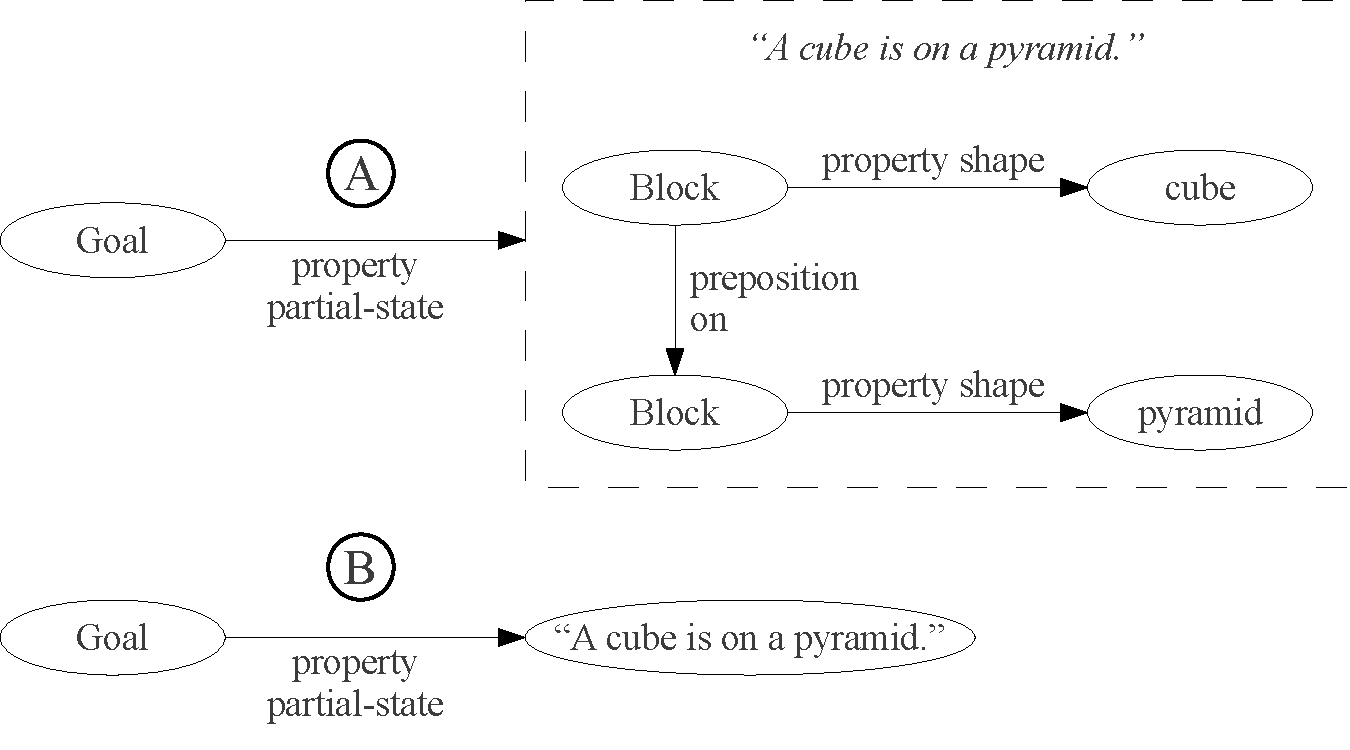
\includegraphics[width=10cm]{gfx/deliberative_physical_partial_state_reification}
\caption[Deliberative physical partial state
  reification.]{Deliberative physical partial state reification.  (A)
  A visualization of the idea that a deliberative goal object can
  refer to a potential partial state of the physical knowledge base.
  (B) The actual representation of a deliberative goal object that has
  a symbolic ``partial-state'' property, the symbolic phrase, ``A cube
  is on a pyramid,'' being a reference to the potential physical
  partial state visualized in (A).  Each planning layer is limited to
  reflecting upon reified symbols that refer to partial states in the
  layer below and not the complexity of the partial states
  themselves.}
\label{figure:deliberative_physical_partial_state_reification}
\end{figure}
Because deliberative knowledge only contains symbols that refer to
physical partial states, this allows the deliberative layer to ignore
the internal details of the physical partial state and simply treat
the goal symbolically.

{\mbox{\autoref{figure:meta_meta_knowledge}}} shows a visualization of
an example of reflective knowledge that references potential
deliberative knowledge, while this potential deliberative knowledge
references potential physical knowledge.
\begin{figure}
\centering
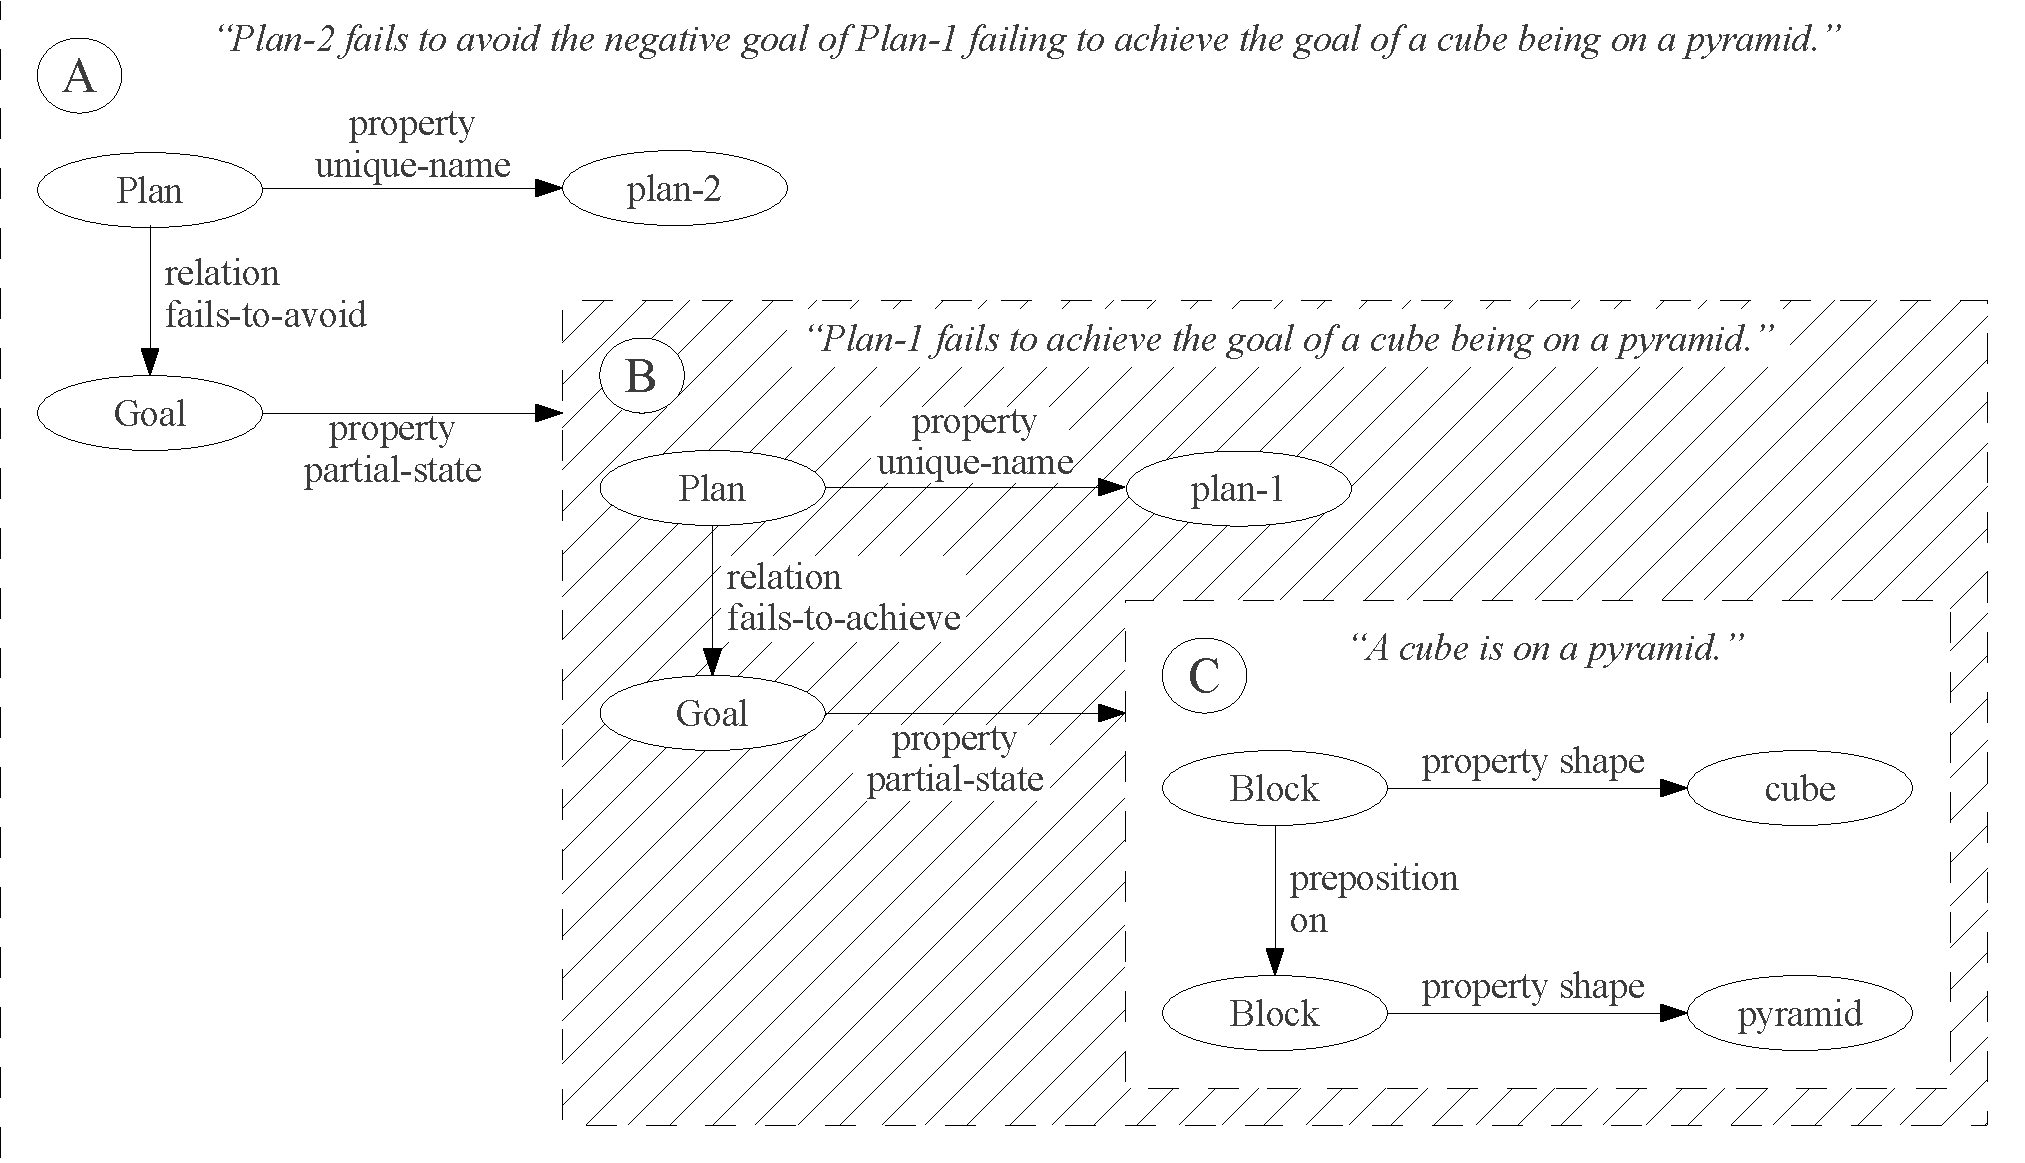
\includegraphics[width=12cm]{gfx/meta_meta_knowledge}
\caption[A visualization of a reflective partial state with references
  to potential knowledge in the layers below.]{A visualization of a
  reflective partial state with references to potential knowledge in
  the layers below.  Although this reflective knowledge is visualized
  as a hyper-graph that includes deliberative and physical knowledge,
  all deliberative and physical knowledge is actually symbolically
  reified in the reflective partial state.  This is not a
  visualization of deliberative knowledge or physical knowledge.  This
  is a visualization of reflective knowledge.}
\label{figure:meta_meta_knowledge}
\end{figure}

\section{The Interpretation Process in Three Layers}

\begin{enumerate}
\item{\emph{Physical Partial State}: ``A pyramid is on a cube.''}
\item{\emph{Deliberative Partial State}: ``A deliberative planner is
  focusing on a plan that is hypothesized to cause a cube to be on a
  pyramid.''}
\item{\emph{Reflective Partial State}: ``A reflective planner is
  focusing on a plan that is hypothesized to cause a deliberative
  planner to be focusing on a plan that is hypothesized to cause a
  cube to be on a pyramid.''}
\end{enumerate}

has the potential to be more complex and thus more difficult to reason
about than the knowledge in the layers below that knowledge.  For
example, a partial state of the physical problem domain can be a
simple relationship such as ``a pyramid being on a cube.''  Since the
deliberative layer contains meta-physical knowledge, or ``knowledge
about physical knowledge,'' a simple deliberative partial state could
be that ``a deliberative plan fails to accomplish the goal for a cube
to be on a pyramid.''  This deliberative knowledge appears at first
glance to be more complex than the physical knowledge that it is about
because it contains, in some sense, the physical knowledge as well as
additional relationships between this physical knowledge and a plan
and a goal.  Further, the reflective layer contains meta-meta-physical
knowledge, so a piece of reflective knowledge could be that ``a
reflective plan fails to avoid the negative goal of a deliberative
plan failing to achieve the goal of a cube being on a pyramid.''
{\mbox{\autoref{figure:meta_meta_knowledge}}} shows a visualization of
this example of meta-meta-knowledge with a reflective partial state
that references a deliberative partial state that references a
physical partial state.
\begin{figure}
\centering
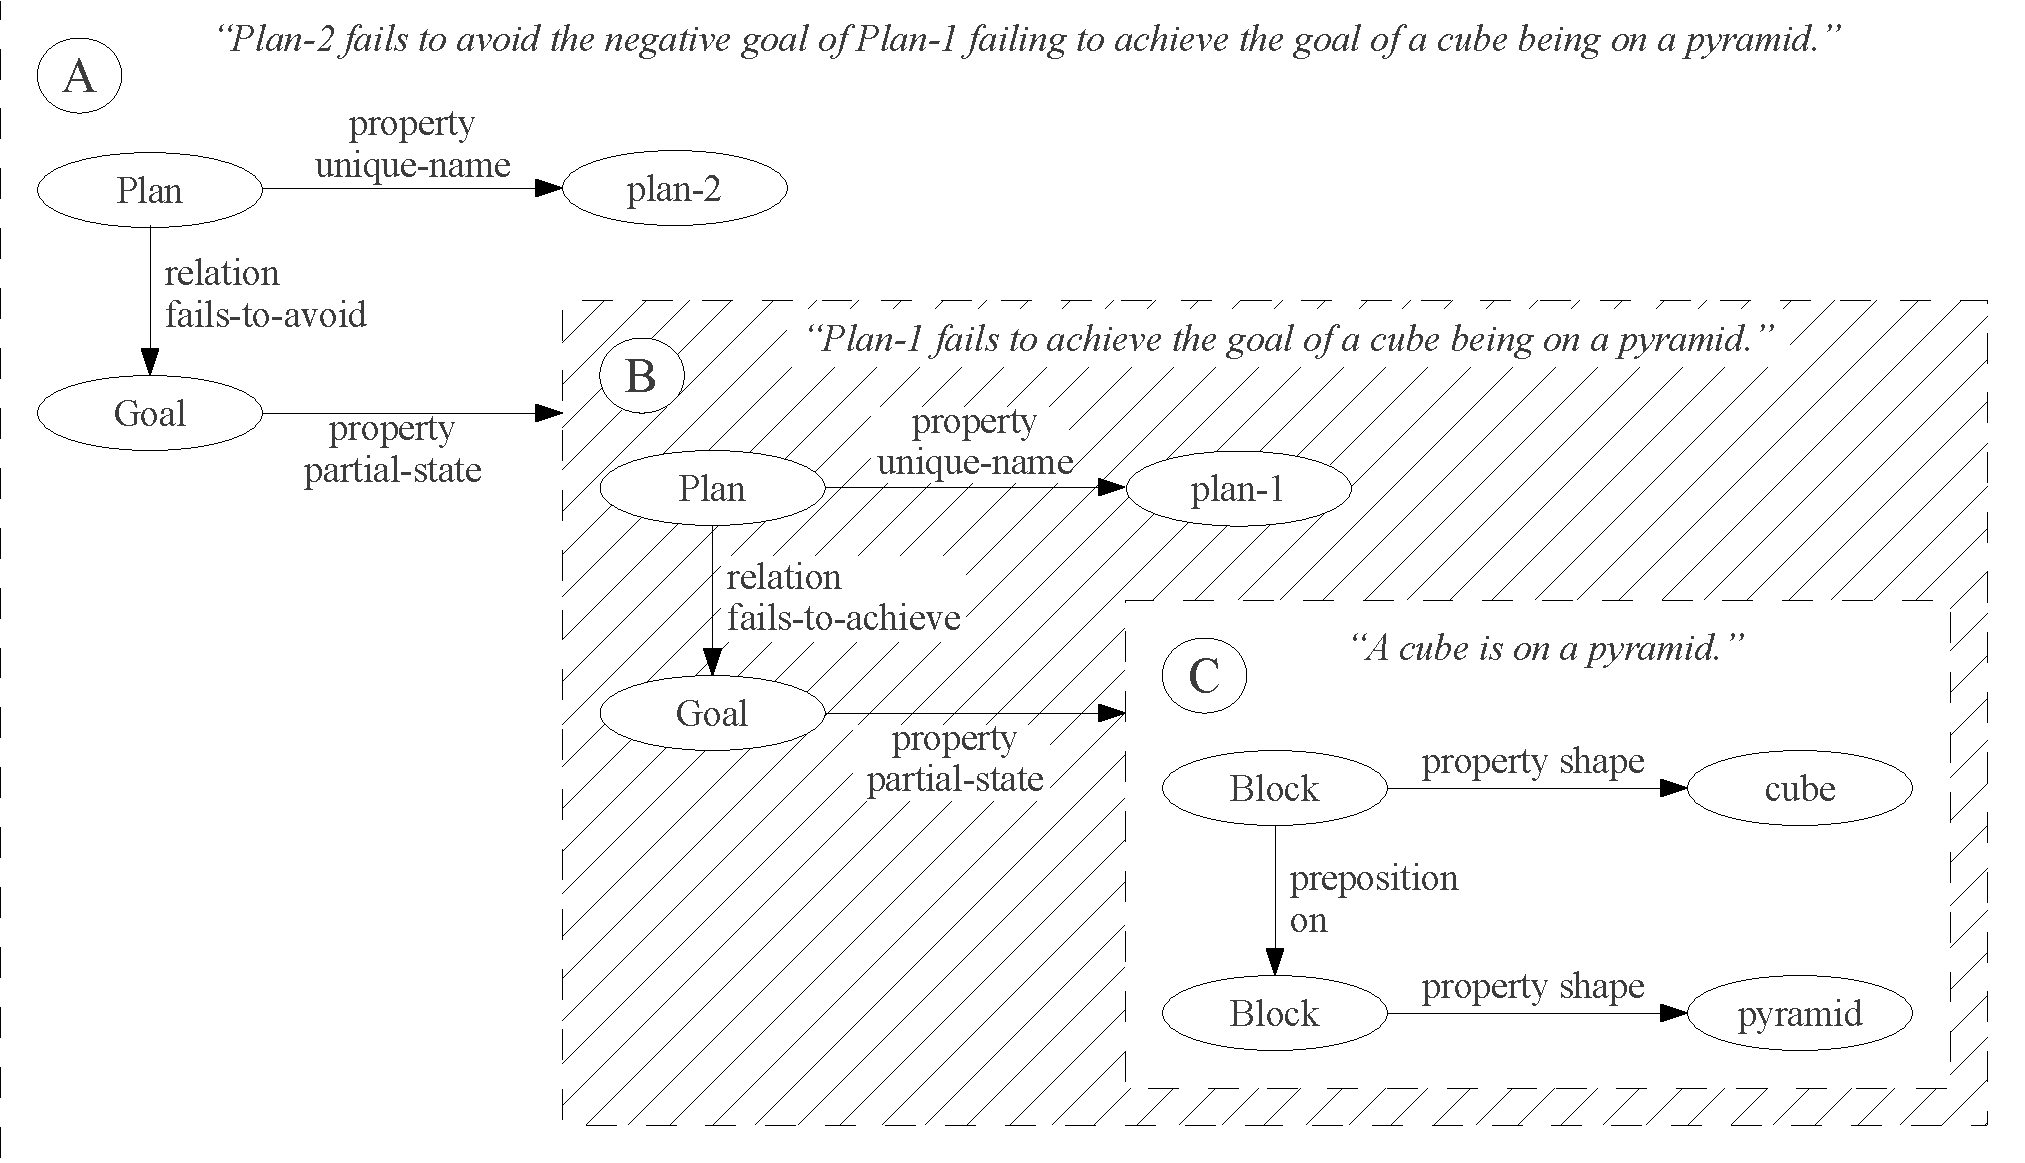
\includegraphics[width=12cm]{gfx/meta_meta_knowledge}
\caption{Meta-meta-knowledge of (A) a reflective partial state that
  references (B) a deliberative partial state that references (C) a
  physical partial state.}
\label{figure:meta_meta_knowledge}
\end{figure}
{\mbox{\autoref{table:meta_meta_knowledge_complexity}}} shows the
computational complexity of evaluating each one of these increasingly
complex forms of knowledge.  The phrase, ``a cube is on a pyramid,''
is interpreted in the deliberative layer and results in the following
SALS program:

\begin{samepage}
\begin{Verbatim}
[exists
  [relationship block property shape 'cube'
                preposition on
                block property shape 'pyramid']]
\end{Verbatim}
\end{samepage}

\noindent The phrase, ``a deliberative planner is focusing on a plan
that is hypothesized to cause a cube to be on a pyramid,'' is
interpreted by the reflective layer and refers to a partial state of
the deliberative plan knowledge base, which results in the following
SALS program:

\begin{samepage}
\begin{Verbatim}
[exists
  [relationship planner property planner_type deliberative
                relation focus_plan
                plan property hypothesized_to_cause
                [relationship block property shape 'cube'
                              preposition on
                              block property shape 'pyramid']]]
\end{Verbatim}
\end{samepage}

\noindent The phrase, ``a reflective planner is focusing on a plan
that is hypothesized to cause a deliberative planner to be focusing on
a plan that is hypothesized to cause a cube to be on a pyramid,'' is
interpreted by the super-reflective layer and refers to a partial
state of the reflective plan knowledge base, which results in the
following SALS program:

\begin{samepage}
\begin{Verbatim}
[exists 
  [relationship planner property planner_type reflective
                relation focus_plan
                plan property hypothesized_to_cause
    [relationship planner property planner_type deliberative
                  relation focus_plan
                  plan property hypothesized_to_cause
                  [relationship block property shape 'cube'
                                preposition on
                                block property shape 'pyramid']]]]
\end{Verbatim}
\end{samepage}



\begin{table}
\centering
\begin{tabular}{|l|c|c|}
\hline
                 &Execution Nodes   &Plan Analogies    \\
                 &{\scriptsize{(Imagine/Execute)}} &{\scriptsize{(Imagine/Execute)}} \\
\hline
Deliberative     & 18/12            & 2/0              \\
\hline
Reflective       & 98/22            & 10/0             \\
\hline
Super Reflective & 348/32           & 27/0             \\
\hline
\end{tabular}
\caption{The number of execution nodes and plan analogies that were
  made interpreting a deliberative statement about physical knowledge,
  a reflective meta-knowledge statement about deliberative knowledge
  that references the same physical knowledge, and a super-reflective
  meta-meta-knowledge statement that references the same physical
  knowledge through deliberative knowledge.}
\label{table:meta_meta_knowledge_complexity}
\end{table}


\begin{table}
\centering
\begin{tabular}{|l|r|r|}
\hline
                 &Execution Nodes &Plan Analogies \\
\hline
Super Reflective & 152            & 11            \\
\hline
Reflective       & 170            & 13            \\
\hline
Deliberative     & 3003           & 240           \\
\hline
\end{tabular}

\begin{tabular}{|l|r|r|}
\hline
                 &Version Spaces &Hypotheses \\
\hline
Super Reflective &               &           \\
\hline
Reflective       &               &           \\
\hline
Deliberative     &               &           \\
\hline
\end{tabular}
\caption{The number of execution nodes and plan analogies that were
  made during in different stages of plan processing in the different
  planning layers during a planning scenario involving the super
  reflective layer interpreting and compiling a plan to ``find and
  execute a recently learned plan that avoids a negative reflective
  goal.''  The execution of the super reflective plan becomes the
  reflective planning process.  The reflective planning process
  searches through deliberative plans until it finds a plan to ``find
  and execute a recently learned plan for accomplishing a positive
  deliberative goal.''  The execution of the reflective plan becomes
  the deliberative planning process.  The deliberative planning
  process interprets and imagines a plan to ``stack a cube on a
  pyramid,'' which is hypothesized to accomplish a positive
  deliberative goal.}
\label{table:plan_interpretation_computational_complexity_of_layers}
\end{table}


\begin{table}
\centering
\begin{tabular}{|l|r|r|}
\hline
                 &Execution Nodes &Plan Analogies \\
\hline
Super Reflective & 152            & 11            \\
\hline
Reflective       & 170            & 13            \\
\hline
Deliberative     & 3003           & 240           \\
\hline
\end{tabular}

\begin{tabular}{|l|r|r|}
\hline
                 &Version Spaces &Hypotheses \\
\hline
Super Reflective &               &           \\
\hline
Reflective       &               &           \\
\hline
Deliberative     &               &           \\
\hline
\end{tabular}
\caption{The number of execution nodes and plan analogies that were
  made during in different stages of plan processing in the different
  planning layers during a planning scenario involving the super
  reflective layer interpreting and compiling a plan to ``find and
  execute a recently learned plan that avoids a negative reflective
  goal.''  The execution of the super reflective plan becomes the
  reflective planning process.  The reflective planning process
  searches through deliberative plans until it finds a plan to ``find
  and execute a recently learned plan for accomplishing a positive
  deliberative goal.''  The execution of the reflective plan becomes
  the deliberative planning process.  The deliberative planning
  process interprets and imagines a plan to ``stack a cube on a
  pyramid,'' which is hypothesized to accomplish a positive
  deliberative goal.}
\label{table:plan_interpretation_computational_complexity_of_layers}
\end{table}

%% \section{Old Stuff}

%% This dissertation consists of four contributions that work together to
%% form the SALS AI.  From the low-level virtual machine and Lisp-like
%% programming language to the reflective and super-reflective layers of
%% the Emotion Machine cognitive architecture, it is difficult to
%% evaluate all aspects of the SALS AI by a single simple metric.
%% Therefore, this chapter presents a number of different metrics that
%% are used to evaluate the four contributions:
%% \begin{packed_enumerate}
%% \item{\emph{Emotion Machine Cognitive Architecture}: The primary
%%   contribution of this thesis is a recursive implementation of a
%%   reflective planning layer that controls a deliberative planning
%%   process.  Because of the recursive nature of the implementation, a
%%   super-reflective layer is also used to control and learn about the
%%   reflective planning process.  The benefit of adding each additional
%%   reflective layer is that more can be learned from each deliberative
%%   failure by adding each additional reflective layer, but there is a
%%   computational trade-off in that each additional reflective layer
%%   also increases the computational complexity of the overall
%%   architecture.  This chapter evaluates the Emotion Machine cognitive
%%   architectural component of the SALS AI by asking the following
%%   question: What is the increase in computational complexity
%%   introduced by adding additional reflective planning layers to the
%%   basic deliberative planning process?}
%% \item{\emph{Learning from Being Told Natural Language Plans}: The
%%   ability of each planning layer in the SALS AI to interpret and
%%   imagine the effects of ambiguous natural language plans relies on a
%%   search through possible interpretations of each natural language
%%   phrase in any given plan.  This search would quickly become
%%   intractable if it were not controlled by a number of different types
%%   of low-level programmatic constraints.  Only those natural language
%%   plan interpretations that make programmatic sense according to these
%%   constraints are further considered for imagination or execution.  In
%%   practice, each low-level constraint helps to reduce the overall
%%   search complexity by varying amounts depending on the domain of
%%   control, whether the natural language plan is describing a control
%%   process for the physical, deliberative, or reflective knowledge
%%   domains.  This chapter shows empirical results that compare the size
%%   of the overall natural language plan interpretation search with and
%%   without each of these constraints for the control of each knowledge
%%   domain in the SALS AI.  This chapter also discusses the trade-offs
%%   between introducing language specific constraints, such as
%%   English-only semantics or syntax, versus purely programmatic
%%   constraints that keep the SALS natural planning language as it is
%%   currently applicable to all natural human languages.}
%% \item{\emph{Learning Asynchronously from Experience}: The ability of
%%   each planning layer in the SALS AI to asynchronously abstract the
%%   partial state events in its control knowledge domain as well as
%%   asynchronously learn rule-based causal models of resource
%%   activations of the layer below introduces two potentially
%%   problematic scaling factors for the computational complexity of the
%%   overall SALS AI.  Firstly, the number of partial states in arbitrary
%%   knowledge domains could in the worst case introduce a factorial
%%   growth with the size of the knowledge domain and the size of the
%%   partial states being abstracted.  As factorial growth would be an
%%   intractable scaling factor for the computational complexity, this
%%   chapter shows empirical evidence for the actual scaling factors for
%%   abstracting partial states from each of the control knowledge
%%   domains, including the physical, deliberative, and reflective
%%   knowledge domains.  The causal hypothesis rule-learning algorithm
%%   could potentially even have a worse scaling factor that is a
%%   multiplier on the number of partial states abstracted in the first
%%   asynchronous stage in the SALS AI's learning from experience.  This
%%   chapter will also present empirical evidence of the actual scaling
%%   factor introduced by the conjunctive rule-learning algorithm
%%   employed in learning causal models of resource activations in the
%%   SALS AI for each planning layer, including the deliberative,
%%   reflective, and super-reflective layers.}
%% \item{\emph{Virtual Machine and Programming Language}: The SALS AI is
%%   constructed on a low-level virtual machine and Lisp-like programming
%%   language that takes advantage of multithreaded and multicore CPUs.
%%   The SALS virtual machine executes concurrent bytecode processes that
%%   are called ``fibers,'' which are an abstraction of the POSIX threads
%%   provided by the underlying operating system.  In order to minimize
%%   hyperthread-specific cache-miss effects for each concurrently
%%   executing fiber, a separate memory pool is allocated for each
%%   hardware hyperthread in each CPU core in the underlying hardware
%%   platform.  The SALS virtual machine performs dynamic load balancing
%%   in order to take advantage of as many CPU cores as possible while
%%   executing multiple fibers.  Also, the SALS virtual machine includes
%%   a concurrent tricolor garbage collection algorithm that has been
%%   optimized to be used over multiple memory pools.  In a perfect
%%   symmetric multiprocessing (SMP) system, executing $N$ fibers on $N$
%%   processors should have a constant time-complexity, but modern
%%   multithreaded and multicore CPUs have shared caches between
%%   hyperthreads and cores, which makes systems based on these CPUs less
%%   than ideal SMPs.  Furthermore, mutual exclusion (mutex) locks
%%   required for garbage collection slow down garbage collection across
%%   multiple memory pools by a factor depending on the number of
%%   cross-references between pools.  This chapter empirically evaluates
%%   how the SALS virtual machine performs at minimizing these cache-miss
%%   and locking effects on an Intel Core i7 CPU, which has 4 cores, each
%%   with 2 hyperthreads, while executing various numbers of concurrent
%%   fibers.}
%% \end{packed_enumerate}

%% \section{Computational Complexity of Reflective Layers}

%% What is the increase in computational complexity introduced by adding
%% additional reflective planning layers to the basic deliberative
%% planning process?  The answer to this question is not at first obvious
%% because of the exponentially larger state-space confronted by each
%% higher planning layer.  The result is that each additional layer adds
%% a roughly linear increase in computational complexity to the overall
%% architecture.  This chapter discusses how the increased computational
%% complexity of each additional reflective planning layer is kept from
%% becoming exponential in the SALS AI.  This chapter also discusses how
%% using concurrent hardware in order to separately simulate each
%% additional reflective layer has the potential to reduce the overall
%% time-complexity of the architecture to sub-linear per additional
%% layer.

%% The SALS AI consists of 100 parallel heterogeneous resources,
%% organized into 29 agencies, which comprise the 5 layers.  The causal
%% procedurally reflective tracing features of the SALS virtual machine
%% that have been described in
%% {\mbox{\autoref{chapter:virtual_machine_and_programming_language}}}
%% allow for the run-time evaluation of each separate causally scoped
%% component of the SALS AI.  In the evaluation of the complexity of each
%% additional reflective layer, the following execution events are
%% measured:
%% \begin{packed_enumerate}
%% \item{Memory Allocation in Bytes}
%% \item{Garbage Collection in Bytes}
%% \item{Bytecode Execution Count}
%% \item{Semantic Frame Slot Mutations}
%% \item{Plan Interpretation Nodes Considered}
%% \item{Analogical Plan Matches Considered}
%% \end{packed_enumerate}
%% Each planning layer in the SALS AI can be used to specify very similar
%% types of goals.  For example, consider the following three different
%% pieces of knowledge:
%% \begin{packed_enumerate}
%% \item{``A pyramid is on a cube.''}
%% \item{``A deliberative planner has the positive goal for a pyramid to
%%   be on a cube.''}
%% \item{``A reflective planner has the positive goal for a deliberative
%%   planner to have the positive goal for a pyramid to be on a cube.''}
%% \end{packed_enumerate}
%% This is the feared, worst-case scenario that the analogical language
%% interpretation process in each subsequently higher reflective layer of
%% reasoning becomes an exponentially more difficult problem.  In
%% general, however, this is not true because reflective reasoning does
%% not and in practice often does not involve directly interpreting these
%% types of exponentially more difficult natural language interpretation
%% problems.  This is because reflective natural language plans are very
%% rarely directly about specific states of knowledge in the physical
%% knowledge base as in these examples.  Usually, reflective knowledge is
%% about much simpler partial states of the deliberative planning machine
%% that do not involve any physical knowledge at all.  For example,
%% consider the following pieces of knowledge:
%% \begin{packed_enumerate}
%% \item{``A deliberative planner is focused on a plan that has failed.''}
%% \item{``A reflective planner is focused on a plan that has failed.''}
%% \end{packed_enumerate}

%% {\mbox{\autoref{table:plan_interpretation_computational_complexity_of_layers}}}
%% shows measures of computational complexity for each planning layer in
%% SALS AI as it goes through the learning scenario presented in the
%% introduction to this dissertation.
%% \begin{table}
%% \centering
%% \begin{tabular}{|l|l|l|l|l|}
%% \hline
%%                  &Alloc &GC &BC &Mutate \\
%% \hline
%% Deliberative     &      &   &   &       \\
%% \hline
%% Reflective       &      &   &   &       \\
%% \hline
%% Super Reflective &      &   &   &       \\
%% \hline
%% \end{tabular}
%% \caption{Computational complexity of plan interpretation for each
%%   planning layer.}
%% \label{table:plan_interpretation_computational_complexity_of_layers}
%% \end{table}
%% In order to measure the increase in computational complexity
%% introduced by adding additional reflective planning layers to the
%% basic deliberative planning process,   While more can be learned from
%% each deliberative failure by adding additional reflective planning
%% layers, each additional reflective layer also increases the
%% computational complexity of the overall architecture.  First, let us
%% consider the computational complexity of the deliberative planning
%% layer.

%% The answer to this question is not at first obvious because of the
%% exponentially larger state-space confronted by each higher planning
%% layer.

%% The result is that each additional layer adds a roughly linear
%% increase in computational complexity to the overall architecture.

%% This chapter discusses how the increased computational complexity of
%% each additional reflective planning layer is kept from becoming
%% exponential in the SALS AI.

%% This chapter also discusses how using concurrent hardware in order to
%% separately simulate each additional reflective layer has the potential
%% to reduce the overall time-complexity of the architecture to
%% sub-linear per additional layer.

%% \section{Computational Scaling of Natural Language Interpretation Constraints}

%% \section{Computational Scaling of Partial State Abstraction and Rule-Learning}

%% Given that each planning layer in the SALS AI is based on perceiving
%% and acting based on the existence or non-existence of partial states
%% in the knowledge base that is being controlled by the planning layer,
%% the state-space of the control domain that is perceived and reacted to
%% by a planning layer is directly related to the number of partial
%% states that can be abstracted from this control domain.  For example,
%% if we consider that the knowledge base that is being controlled by a
%% given planning layer is represented as a graph, which is not exactly
%% correct but will suit our purposes here, the set of partial states
%% that can be abstracted from this control domain includes a subset of
%% all possible subgraphs of this graph representation.  In order to
%% avoid an intractable number of partial states being automatically
%% abstracted from a given knowledge base, the types of partial states
%% that the SALS AI abstracts are limited to the ``relationship'' and
%% ``property'' types of partial states described in
%% {\mbox{\autoref{chapter:learning_asynchronously_from_experience}}}.
%% These simple types of partial states limit the complexity



%% %\begin{equation}
%% %({2^n}-1)\left(\frac{n(n-1)}{2}\right)^{\ell}
%% %\end{equation}


%% \section{Computational Scaling of Concurrent Processing Hardware}


%% \section{old stuff}

%% \section{Boot-up and Perceive Experiment}

%% As an initial evaluation of the run-time performance of the AI, I have
%% run an experiment that simply initializes the AI and lets it perceive
%% the world over time.  The physical world does not change during this
%% experiment and the AI is not given any goals to accomplish, so this
%% experiment is a control that shows the baseline memory usage and
%% run-time performance of the cognitive architecture in its ``idling''
%% mode.  This experiment shows that the mind takes $10$ minutes to
%% initialize.  After initializing, the AI learns from its initial
%% perception and continues to attempt to detect changes in its raw
%% visual input over the next $50$ minutes.  Over the $50$ minutes of
%% continuous perception, the mind uses a highly fluctuating amount of
%% memory that stays, on average, relatively constant.  The mind is not
%% static in this experiment.  The mind contains resources that allocate
%% an average of $1.8$ megabytes per second in the built-in reactive
%% layer process of detecting visual changes in the next state from the
%% physical simulation, so that these changes may be propagated to the
%% physical knowledge of the learned reactive layer in a stream of
%% events.  Over $6$ gigabytes of memory is allocated over the entire
%% $60$ minutes of the experiment.  The mind uses an average memory
%% footprint of about $26$ megabytes over the course of the experiment.
%% The bytecode execution rate stabilizes at about $12$ thousand
%% bytecodes per second.  The concurrent processing capabilities of the
%% architecture can handle bursts of $50$ thousand bytecodes per second,
%% but this experiment simply shows that the execution rate of the
%% architecture does not slow down over time.  The entire cognitive
%% architecture exhibits stable handling of continuous processing for
%% experiments lasting over an hour, handling the allocation and garbage
%% collection of many gigabytes of memory in the process.
%% {\mbox{\autoref{figure:data/bootup_evaluation/mind_plot-Gripper-1}}}
%% shows a plotted overview of the run-time performance of the AI during
%% the boot-up and perceive experiment.  \autoref{table:bootup} on page
%% \pageref{table:bootup} shows more detailed plots for the run-time
%% behavior of each individual layer and agency within the AI.
%% %\experimentAIdatafigures[60]{bootup_evaluation}{an experiment that
%% %  boots up the AI, allowing it to continue to perceive the physical
%% %  world over time without stimulating it to achieve any goals.  This
%% %  experiment shows that the AI learns from its initial perceptions,
%% %  and when these do not change, it has nothing to learn and memory
%% %  usage is stable.}

%% \section{Deliberative Learning Experiment without Reflection}

%% The second run-time experiment that was performed with the cognitive
%% architecture does not include the reflective learning component that
%% learns hypothetical models for how the deliberative resources modify
%% the planning machine type knowledge base.  The AI is initialized,
%% which takes the same $10$ minutes as in the initial experiment.  The
%% AI is then told to execute a deliberative plan, which causes it to
%% execute a plan that attempts to stack a cube on top of a pyramid.  In
%% learning the effects of reactive resource executions on the physical
%% type knowledge bases the deliberative AI allocates $5.3$ megabytes per
%% second, while the memory footprint only grows at a rate of $90$
%% thousand bytes per second due to the learning that occurs over the
%% $60$ minutes that it takes to fail to accomplish this goal.  The AI
%% does not respond to the failure because the reflective layers are not
%% active.  The AI allocates an average of $1.2$ megabytes of memory per
%% second for the length of the experiment, which results in a total of
%% $5.4$ gigabytes over the course of the experiment.  The architecture
%% executes an average of $11$ thousand bytecodes per second over the
%% course of the experiment.  This shows that the architecture slows down
%% when more resources are active than simply the reactive perceptual
%% resources.  As deliberative learning resources become active, the
%% bytecode rate does not decrease much from the $12$ thousand bytecodes
%% per second in the control, but the overall memory allocation rate does
%% decrease by a factor of $66$\% from $1.8$ megabytes per second in the
%% control to $1.2$ megabytes per second with deliberative learning
%% enabled.
%% {\mbox{\autoref{figure:data/no_reflective_learning_evaluation/mind_plot-Gripper-1}}}
%% shows a plotted overview of the run-time performance of the AI during
%% the deliberative learning experiment with the reflective layer
%% disabled.  \autoref{table:no_reflective_learning} on page
%% \pageref{table:no_reflective_learning} shows plots of data for the
%% entire mind, each layer, as well as each agency within each layer for
%% this deliberative learning experiment.
%% %\experimentAIdatafigures[75]{no_reflective_learning_evaluation}{an
%% %  experiment with the reflective tracing of the deliberative process
%% %  disabled.  This experiment can be compared with run-time behavior of
%% %  the full AI cognitive architecture, which can learn from the failure
%% %  and initiate a second attempt at plan selection and execution.}

%% \section{Deliberative and Reflective Learning Experiment (The Full Architecture)}

%% The third run-time experiment that was performed with the cognitive
%% architecture includes both the deliberative as well as reflective
%% learning layers.  The deliberative layer learns hypothetical models of
%% the reactive resource execution effects on the physical type knowledge
%% base, while the reflective layer learns hypothetical models of the
%% deliberative resource execution effects on the deliberative planning
%% machine type knowledge base.  Although this experiment involves an
%% initial imaginative and plan selection processes in the reflective
%% layer, this experiment runs very similarly through the first $75$
%% minutes of otherwise mostly deliberative and reactive resource
%% executions.  Around minute $75$, the cognitive architecture responds
%% to the failure in the deliberative planning machine with the
%% reflective bug response, which begins another round of reflective
%% learning, imagination, and refined plan selection.  After a reflective
%% bug response, the goal is accomplished successfully around minute
%% $105$.  The experiment is allowed to run continuously after this point
%% for a total of $180$ minutes in order to show the performance of
%% baseline perceptual activity after going through the complete process
%% of deliberative and reflective learning.  Except for a blip at minute
%% $135$, which requires an extended garbage collection period, the AI is
%% otherwise stable after both layers have successfully demonstrated
%% learning.  With the addition of the reflective learning layer in the
%% final experiment the average bytecode execution rate has dropped
%% significantly, running at a factor $55$\% of the execution rate of the
%% architecture in the experiment demonstrating only deliberative
%% learning.  This experiment demonstrates the taxing demand of the extra
%% concurrent processes and memory allocation required with the
%% additional reflective learning algorithm.  However, slowing the
%% algorithm down by a factor of two with the addition of a reflective
%% layer of learning shows that the slow down is roughly linear with the
%% additional layer.  For example, in a naive approach to reflective
%% learning, an exponential increase in processing would be expected
%% because all resource executions and knowledge in the layers below
%% would be reflected upon and modelled by the reflective layer.  Because
%% the reflective learner implemented in this architecture only reflects
%% over the deliberative planning machine and not all of the processing
%% in the layers below, this architecture shows a linear slowdown with
%% the addition of reflective layers of learning.
%% {\mbox{\autoref{figure:data/reflective_learning_evaluation/mind_plot-Gripper-1}}}
%% shows a plotted overview of the run-time performance of the AI during
%% the reflective learning experiment.
%% \autoref{table:reflective_learning} on page
%% \pageref{table:reflective_learning} shows plots of data for the entire
%% mind, each layer, as well as each agency within each layer for this
%% reflective learning experiment, showing the run-time performance of
%% the full architecture.
%% %\experimentAIdatafigures[180]{reflective_learning_evaluation}{an
%% %  experiment testing the full AI cognitive architecture, including the
%% %  reflective tracing of the deliberative planning process, imagining
%% %  the potential failures of the deliberative planning machine as well
%% %  as the physical effects of physical actions.}

%% \section{No Theoretical Slowdown of Original Algorithm}

%% In order to assume that there is no theoretical slowdown of the
%% original planning algorithm when reflective learning is applied, it
%% must be assumed that the reflective implementation is an ideal
%% concurrent shared memory architecture.  In practice, the underlying
%% Funk virtual operating system slows down when more concurrent and
%% parallel tasks are executing.  This is beside the theoretical point,
%% but the following table shows a real-time test of the actual slowdown
%% experienced by the Funk operating system as different numbers of
%% parallel tasks are executed to perform a simple numerical processing
%% task.  The test was done on a dual Pentium processor computer, each
%% with ``core duo'' technology with each core implementing
%% ``hyper-threading'', which ends up appearing as eight processors to
%% the Linux operating system underlying the Funk virtual operating
%% system:

%% \vspace{5mm}
%% \begin{tabular}{ll}
%% Tasks & Real-Time (s) \\
%% 1 & 29\\
%% 2 & 36\\
%% 3 & 46\\
%% 4 & 44\\
%% 5 & 68\\
%% 6 & 67\\
%% 7 & 73\\
%% 8 & 110\\
%% \end{tabular}
%% \vspace{5mm}

%% As each additional concurrent resource in the cognitive architecture
%% begins execution, this table shows the approximate slowdown that the
%% Funk virtual machine experiences on this specific dual processor
%% hardware.

